\documentclass[11pt]{article}
\usepackage[letterpaper,margin=0.84in]{geometry}
\usepackage[T1]{fontenc}
\usepackage{lmodern,microtype}
\usepackage{amsmath,amssymb,amsthm,mathtools,bm}
\usepackage{booktabs,array,longtable,graphicx,caption,subcaption,enumitem,xcolor,float}
\newcolumntype{L}[1]{>{\raggedright\arraybackslash}p{#1}}
\usepackage{hyperref}
\usepackage[nameinlink,capitalise]{cleveref}
\usepackage{fancyhdr,titlesec}
\hypersetup{
 colorlinks=true,
 linkcolor=blue!55!black,
 citecolor=blue!55!black,
 urlcolor=blue!55!black,
 pdftitle={Exact Two-Block QGN Stiffness, Twist-Covariance Obstructions, and Interaction-Defined Subbundles},
 pdfauthor={Nicholas Sledgianowski}
}
\pagestyle{fancy}
\fancyhf{}
\fancyhead[L]{\small Two-block QGN stiffness and covariance audit}
\fancyhead[R]{\small Reviewer-corrected draft -- July 25, 2026}
\fancyfoot[C]{\thepage}
\setlength{\headheight}{14pt}
\titleformat{\section}{\large\bfseries}{\thesection.}{0.5em}{}
\titleformat{\subsection}{\normalsize\bfseries}{\thesubsection.}{0.5em}{}
\setlist[itemize]{leftmargin=1.5em,itemsep=0.22em,topsep=0.35em}
\setlist[enumerate]{leftmargin=1.7em,itemsep=0.22em,topsep=0.35em}
\allowdisplaybreaks
\newtheorem{theorem}{Theorem}[section]
\newtheorem{proposition}[theorem]{Proposition}
\newtheorem{corollary}[theorem]{Corollary}
\newtheorem{lemma}[theorem]{Lemma}
\theoremstyle{remark}
\newtheorem{remark}[theorem]{Remark}
\newcommand{\Tr}{\operatorname{Tr}}
\newcommand{\rank}{\operatorname{rank}}
\newcommand{\spec}{\operatorname{spec}}
\newcommand{\ket}[1]{\lvert #1\rangle}
\newcommand{\bra}[1]{\langle #1\rvert}
\newcommand{\I}{\mathrm i}
\newcommand{\e}{\mathrm e}
\newcommand{\Id}{\mathbb I}
\newcommand{\cH}{\mathcal H}
\newcommand{\cK}{\mathcal K}
\newcommand{\cV}{\mathcal V}
\newcommand{\cZ}{\mathcal Z}
\newcommand{\cS}{\mathcal S}
\newcommand{\cQ}{\mathcal Q}
\newcommand{\bmA}{\bm A}
\newcommand{\bmk}{\bm k}
\newcommand{\bmR}{\bm R}
\newcommand{\bmQ}{\bm Q}

\title{\textbf{Exact Two-Block QGN Stiffness and Twist-Covariance Obstructions}\\[0.35em]
\large Displacement-Balanced Pair Transfer and Interaction-Defined Subbundles in Twisted WSe$_2$}
\author{Nicholas Sledgianowski}
\date{July 25, 2026}

\begin{document}
\maketitle

\begin{abstract}
We develop a two-block quantum-geometric-nesting (QGN) framework that cleanly separates exact blockwise stiffness, physical electromagnetic twisting, and composition-space mixing.  A translation-invariant projected lattice model has two extensive pseudospin blocks, an exact rank-two one-pair reduction in each block, inverse pair masses $U/16$ and $5U/8$, and a composition-relaxed ground-energy envelope with an exact middle-filling zero despite positive mobility in both blocks.

We then audit two proposed mechanisms for ordinary-twist composition hopping.  A momentum-dependent common unitary contributes only a removable commutator source.  More importantly, a multi-site active--remote bridge must itself be Peierls twisted.  When its kernel is shifted consistently with the active projector, $P(\bm A)B(\bm A)P(\bm A)$ is a covariance orbit of its zero-twist value, and a projected zero row remains identically zero.  The nonzero derivative obtained by holding $B$ fixed is therefore not a physical electromagnetic source.

The correction exposes a sharper surviving structure.  A fermionic monomial is invariant under a uniform Peierls twist precisely when its net covering-lattice displacement vanishes.  The quadrature anisotropy $P_{\rm ph}=g_Y^2-g_X^2$ multiplies exactly the pair-transfer component $X^2+X^{\dagger2}$, and position-balanced pair-hop vertices such as $c_{1x}^\dagger c_{1x'}^\dagger c_{2x'}c_{2x}$ are exactly twist invariant while allowing $P_{\rm ph}\ne0$.  Conditional on a legitimate microscopic transfer source, the exact Jacobi reduction remains valid.  Its bridge-only middle-filling operator has an exact zero mode whenever either quadrature vanishes.  With the positive blockwise QGN curvature included, its thermodynamic middle-filling stiffness is
\[
 \frac18\min\left\{g_X^2+g_Y^2,\ \min(g_X^2,g_Y^2)+\frac94U\right\},
\]
which becomes $(g_X^2+g_Y^2)/8=J/8$ in the endpoint-localized regime.

Finally, we reclassify the twisted-WSe$_2$ calculations.  Active--remote geometry and interaction-defined singular subbundles remain useful gauge-invariant screening diagnostics, but the previously reported $\Gamma_i$ is a geometric proxy rather than a demonstrated source coefficient.  The published $U,V,J$ tensor gives equal transfer quadratures, while a separate position-balanced pair-hop is symmetry allowed but not yet extracted.  A three-band scan still identifies a provisional low-angle design direction, whereas a stricter four-band scan does not establish a controlled material realization.
\end{abstract}

\begin{quote}\small
\textbf{Status and claim hierarchy.}
The block-preserving QGN model, its displacement-resolved Peierls lift, pair masses, trace cancellation, and composition-relaxed envelope are exact.  The common-unitary cancellation, the covariant bridge cancellation, the net-displacement criterion for many-fermion vertices, the quadrature decomposition, and the conditional Jacobi spectral results are analytic.  The compact bridge is now used as a covariance counterexample: its fixed-kernel derivative is nonzero, but its consistently twisted derivative cancels.  The WSe$_2$ sections are numerical screens.  Their $\Gamma_i$ values are explicitly labeled geometric proxies, and no physical composition-hopping coefficient is claimed without a source derived from the fully covariant microscopic interaction.
\end{quote}

\section{Introduction}

Quantum geometric nesting supplies a systematic way to construct frustration-free flat-band Hamiltonians with exact ordered ground states and, in favorable superconducting examples, analytically accessible phase stiffness~\cite{han2024}.  The relation between pair mobility and many-body stiffness has also become a target for rigorous numerical bounds~\cite{gao2026}.  A central difficulty appears as soon as the pairing form has more than one extensive singular or pseudospin block.  The zero manifold then contains many product antisymmetrized geminal powers (AGPs), one for each allowed block composition.  A physical electromagnetic twist may either preserve those compositions, producing a lower envelope of independent branches, or mix them, producing a finite operator on the lattice of compositions.

The companion one-block work established an exact finite-size reduction for a flat-band QGN model and closed the projected-Hubbard Model-II pair-mass calculation~\cite{parent}.  The multi-block addendum derived product-pseudospin irreducibility, center and determinant-resonance criteria, the block-preserving filling law, and the general positive composition-space operator $Q_i=T_i^\dagger T_i$~\cite{addendum}.  The present paper asks for the missing physical construction:
\begin{quote}
Can an ordinary uniform electromagnetic twist, introduced before projection through microscopic Peierls phases, generate nonzero hopping between two extensive QGN block compositions in a local lattice model?
\end{quote}

This question has acquired material relevance because superconductivity is now observed in twisted bilayer WSe$_2$ over a range of twist angles~\cite{xia2025,guo2026}.  Several local three-orbital and directly Wannierized models have been proposed for the $3.65^\circ$ device~\cite{kim2025,tuo2025}, while a relaxation-aware continuum model predicts a second flat Chern band near $2^\circ$ and is transferable over approximately $2^\circ$--$5^\circ$~\cite{zhang2025}.  These systems naturally contain multiple low-energy and remote orbitals, precisely the setting in which an active--remote geometric bridge can occur.

The paper reaches five conclusions.
\begin{enumerate}
\item A fully specified block-preserving projected lattice model has positive pair mass in each block but an exact zero in the composition-relaxed ground-energy envelope at one block capacity.
\item A shared smooth momentum-dependent unitary cannot generate physical composition hopping: its commutator source is removed by the same least-squares projection that defines the curvature.
\item A band-filtered multi-site bridge also fails when Peierls twisted consistently.  Its apparent fixed-kernel source cancels against the derivative of the bridge kernel itself.
\item The physically robust remnant is a displacement-balance law.  Position-balanced four-fermion pair hops are exactly twist invariant and can carry a nonzero pair-transfer anisotropy $P_{\rm ph}$ without violating gauge covariance.
\item Interaction-defined singular subbundles remain a better block basis than individual WSe$_2$ energy bands, but the present scans establish only geometric and block-isolation diagnostics, not a material ordinary-twist source.
\end{enumerate}

\begin{table}[t]
\centering
\caption{Logical status of the principal results after the twist-covariance audit.}
\label{tab:status}
\begin{tabular}{@{}L{0.31\linewidth}L{0.21\linewidth}L{0.40\linewidth}@{}}
\toprule
Result & Status & Qualification\\
\midrule
Two-block Peierls-lifted QGN model & Exact & Band-projected effective Hamiltonian; two independent pseudospins\\
Pair masses and trace cancellation & Exact & Every rectangular torus with $N_x,N_y\ge3$\\
Composition-relaxed middle zero & Exact & Ground-energy envelope; not a dynamical relaxation theorem\\
Common-unitary cancellation & Exact & Applies to a shared analytic dressing of all factor rows\\
Covariant one-body bridge cancellation & Exact & Applies when both $P(\bm A)$ and the multi-site kernel $B(\bm A)$ are Peierls twisted\\
Net-displacement and quadrature laws & Exact & Termwise covering-lattice statement for many-fermion vertices\\
Conditional Jacobi operator & Exact & Algebraic source-Gram reduction; does not by itself construct the source\\
$3.65^\circ$ WSe$_2$ screen & Numerical: negative & Geometry exists, but source covariance, block preservation, and scale separation fail\\
Low-angle interaction-SVD window & Numerical: provisional & Three-band diagnostic; not robustly confirmed by a four-band screen\\
\bottomrule
\end{tabular}
\end{table}

\section{Multi-block curvature framework}
\label{sec:framework}

Let a positive-square projected Hamiltonian depend analytically on the electronic vector potential $\bmA$,
\begin{equation}
H(\bmA)=\frac12\sum_\lambda S_\lambda(\bmA)^\dagger S_\lambda(\bmA),
\label{eq:positive-square-general}
\end{equation}
and let $D(\bmA)$ be the column map collecting all factor rows.  At zero twist, let $\cZ_n=\ker D(0)$ be the exact zero manifold at total pair number $n$.  Write
\begin{equation}
B_i=\left.\partial_{A_i}D(\bmA)\right|_{0},
\qquad
\Pi=P_{\ker D(0)^\dagger}.
\end{equation}
The least-squares curvature map and exact second-order operator on the zero manifold are
\begin{equation}
T_i=\Pi B_i\big|_{\cZ_n},
\qquad
Q_i^{(n)}=T_i^\dagger T_i\succeq0.
\label{eq:target-map}
\end{equation}
For a directional twist $\bmA=t\bm v$, one replaces $B_i$ by $B_v=\sum_i v_iB_i$.  When the electronic twist moves the two constituents of a time-reversed pair by the same $\bmA$, the pair momentum is $\bmQ=2\bmA$.  We use the stiffness normalization
\begin{equation}
D_{s,i}^{\rm gs}(n)=\frac{1}{4V}\lambda_{\min}\!\left(Q_i^{(n)}\right).
\label{eq:stiffness-normalization}
\end{equation}
The superscript ``gs'' emphasizes that this is the curvature of the lowest analytic ground-energy branch after resolving any degeneracy in $\cZ_n$.

For two capacity-$V$ blocks, the product AGP basis is
\begin{equation}
\ket{n_1,n_2}
=\prod_{a=1}^2
\left[\frac{(V-n_a)!}{n_a!V!}\right]^{1/2}
(\eta_a^+)^{n_a}\ket0,
\qquad 0\le n_a\le V.
\label{eq:product-agp-general}
\end{equation}
At fixed total pair number $n$, write $r=n_1$ and $n_2=n-r$.  A block-preserving source makes $Q_i^{(n)}$ diagonal in $r$.  A one-body source that transfers a fermion between blocks changes the pair composition by at most one, so $Q_i^{(n)}$ is a Jacobi matrix.  The universal hard-core coefficients are
\begin{align}
\tau_{1\leftarrow2}(r)&=\frac{(n-r)(V-r)}{V},
&
\tau_{2\leftarrow1}(r)&=\frac{r(V-n+r)}{V},
\label{eq:directed-transfer}\\
\chi_r^{(n)}&=\frac1V
\sqrt{(n-r)(V-r)(r+1)(V-n+r+1)}.
\label{eq:clebsch-transfer}
\end{align}
These factors will recur in both the exact lattice prototype and the material reduction.

\section{An exact block-preserving Peierls-lifted model}
\label{sec:base-model}

\subsection{Flat-band Hamiltonian and projected interaction}

Let
\begin{equation}
\Lambda_{\bm N}=\mathbb Z_{N_x}\times\mathbb Z_{N_y},
\qquad V=N_xN_y,
\qquad N_x,N_y\ge3.
\end{equation}
Each cell contains two sectors $a=1,2$, two internal orbitals $\mu=1,2$, and spin $s=\uparrow,\downarrow$.  Define
\begin{equation}
\alpha_a(\bmk)=\xi_a(\cos k_x+\cos k_y),
\qquad \xi_1=\frac12,
\qquad \xi_2=1,
\end{equation}
with the spin-dependent Bloch Hamiltonians
\begin{equation}
h_{a,s}(\bmk)
=-t\left[\sigma_x\sin\alpha_a(\bmk)
+s\,\sigma_y\cos\alpha_a(\bmk)\right].
\label{eq:modelII-bloch}
\end{equation}
The spectrum is exactly $\{-t,+t\}$.  A smooth lower-band gauge is
\begin{equation}
u_{a,\uparrow}(\bmk)=\frac1{\sqrt2}
\begin{pmatrix}
\e^{\I\alpha_a(\bmk)/2}\\
\I\e^{-\I\alpha_a(\bmk)/2}
\end{pmatrix},
\qquad
u_{a,\downarrow}(\bmk)=u_{a,\uparrow}^*(-\bmk).
\label{eq:modelII-spinor}
\end{equation}
Both orbital weights are pointwise $1/2$.  The real-space hopping and projector coefficients are super-exponentially localized by the Jacobi--Anger expansion.

Let $p_x^a=P_a\ket{x,a}\!\bra{x,a}P_a$ be the projected rank-one frame element and
\begin{equation}
D_x^a=d\Gamma_{a,\uparrow}(p_x^a)
-d\Gamma_{a,\downarrow}(\overline{p_x^a}).
\end{equation}
Choose
\begin{equation}
W=\begin{pmatrix}1&1\\1&2\end{pmatrix},
\qquad
K=W^{\mathsf T}W=
\begin{pmatrix}2&3\\3&5\end{pmatrix},
\end{equation}
and define
\begin{equation}
H_{\rm QGN}=\frac U2\sum_{x,\ell}
\left(\sum_{a=1}^2W_{\ell a}D_x^a\right)^2.
\label{eq:base-QGN}
\end{equation}
The cross term $3U\sum_xD_x^1D_x^2$ is a genuine interblock density interaction, although $N_1$ and $N_2$ remain separately conserved.

Each block has an exact pseudospin generated by
\begin{equation}
\eta_a^+=\sum_{\bmk}
 d_{\bmk a\uparrow}^\dagger d_{-\bmk a\downarrow}^\dagger.
\end{equation}
One may choose the global pairing generator $\eta_F^+=\eta_1^++2\eta_2^+$, corresponding to the form $F=J_1\oplus2J_2$.  The relative coefficient is a choice inside the enlarged product-pseudospin symmetry; it is not dynamically selected by~\eqref{eq:base-QGN}.  For $N_x,N_y\ge3$, the projected frames are connected and nonsynchronized, the joint constraint algebra is $\mathfrak u(V)_1\oplus\mathfrak u(V)_2$, and the even-sector zero space is exactly the product-AGP span.  Its total-$2n$ nullity is
\begin{equation}
Z_{2n}=[z^n](1+z+\cdots+z^V)^2
=\begin{cases}
n+1,&0\le n\le V,\\
2V-n+1,&V\le n\le2V.
\end{cases}
\label{eq:base-nullity}
\end{equation}

\subsection{Physical Peierls lift}

A hopping with covering-lattice displacement $\bm d$ is twisted before projection as
\begin{equation}
T(\bm d;\bmA)=T(\bm d)\e^{-\I\bmA\cdot\bm d}.
\label{eq:peierls-cover}
\end{equation}
On a finite torus the displacement class $\bar{\bm d}$ is lifted by
\begin{equation}
T_{\bm N}(\bar{\bm d};\bmA)
=\sum_{\bm m\in\mathbb Z^2}
T_\infty(\bar{\bm d}+\bm m\odot\bm N)
\e^{-\I\bmA\cdot(\bar{\bm d}+\bm m\odot\bm N)}.
\label{eq:torus-lift}
\end{equation}
The unreduced displacement is essential: an untwisted alias sum does not determine its first and second displacement moments.  For the present embedding,
\begin{equation}
h_{a,s}(\bmk;\bmA)=h_{a,s}(\bmk+\bmA),
\qquad
\bmQ=2\bmA.
\end{equation}
Peierls phases do not change sector endpoints, so the entire base family preserves both block compositions.

\subsection{Exact pair branches and masses}

Restricting to one pair in block $a$ gives the rank-two Hamiltonian
\begin{equation}
H_{{\rm pair},a}(\bmQ)
=UK_{aa}\left[\frac12\Id_V
-\frac1V\sum_{\mu=1}^2
\ket{g_{a,\mu,\bmQ}}\!\bra{g_{a,\mu,\bmQ}}\right],
\end{equation}
where
\begin{equation}
g_{a,1,\bmQ}(\bmk)=\frac12\e^{-\I\delta\alpha_{a,\bmk}(\bmQ)/2},
\quad
g_{a,2,\bmQ}(\bmk)=\frac12\e^{+\I\delta\alpha_{a,\bmk}(\bmQ)/2},
\end{equation}
and
\begin{equation}
\delta\alpha_{a,\bmk}(\bmQ)
=\alpha_a(\bmk+\bmQ/2)-\alpha_a(\bmk-\bmQ/2).
\end{equation}
The two-column Gram matrix has off-diagonal form factor
\begin{equation}
F_{a,\bm N}(\bmQ)=\frac1V\sum_{\bmk}
\e^{\I\delta\alpha_{a,\bmk}(\bmQ)},
\end{equation}
so the exact lowest branch is
\begin{equation}
E_{{\rm pair},a}(\bmQ)
=\frac{UK_{aa}}4\left[1-|F_{a,\bm N}(\bmQ)|\right].
\label{eq:base-pair-branch}
\end{equation}
The finite-grid identities $V^{-1}\sum_{\bmk}\sin k_i=0$ and
$V^{-1}\sum_{\bmk}\sin k_i\sin k_j=\delta_{ij}/2$ give
\begin{equation}
(m^{-1}_{{\rm pair},a})_{ij}
=\frac{UK_{aa}\xi_a^2}{8}\delta_{ij},
\end{equation}
and therefore
\begin{equation}
\boxed{
 m^{-1}_{{\rm pair},1}=\frac U{16}\Id_2,
 \qquad
 m^{-1}_{{\rm pair},2}=\frac{5U}{8}\Id_2.}
\label{eq:base-masses}
\end{equation}
In the thermodynamic limit,
\begin{equation}
F_{a,\infty}(\bmQ)=
J_0\!\left(2\xi_a\sin\frac{Q_x}{2}\right)
J_0\!\left(2\xi_a\sin\frac{Q_y}{2}\right).
\end{equation}

\begin{figure}[t]
\centering
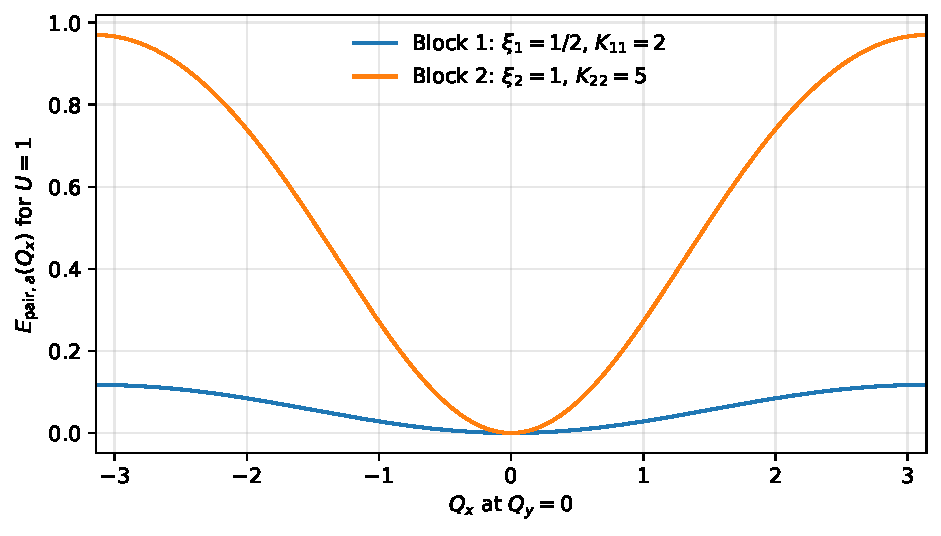
\includegraphics[width=0.78\linewidth]{figures/pair_branches.pdf}
\caption{Exact thermodynamic one-pair branches along $Q_y=0$ for the two block-preserving sectors.  Both branches are mobile, but block 2 has ten times the inverse mass of block 1.}
\label{fig:base-pair-branches}
\end{figure}

\subsection{Trace cancellation and the equilibrium envelope}

The orbital weight symbols satisfy
\begin{equation}
\omega_{a1}(\bmk)=\omega_{a2}(\bmk)=\frac12.
\end{equation}
Hence every paired trace symbol and every finite-volume winding source vanish separately in every block and channel.  With
\begin{equation}
\rho_V(r)=\frac{r(V-r)}{V-1},
\end{equation}
the exact electronic-twist curvature at fixed composition is
\begin{equation}
C_{ij}^{(n_1,n_2)}
=4\sum_{a=1}^2\rho_V(n_a)
(m^{-1}_{{\rm pair},a})_{ij}.
\label{eq:fixed-composition-curvature}
\end{equation}
If the relative block charge is externally fixed, this is the measured static branch.  If only total pair number is equilibrated, the ground-energy curvature is the lower envelope
\begin{equation}
C_{ij}^{\rm gs}(n)=
\min_{n_1+n_2=n}C_{ij}^{(n_1,n_2)}.
\label{eq:equilibrium-envelope}
\end{equation}
The objective is concave in $n_1$, so a minimizing composition has at most one partially filled block.  Since block 1 is the less stiff block,
\begin{equation}
(n_1^*,n_2^*)=
\begin{cases}
(n,0),&0\le n<V,\\
(V,0)\text{ or }(0,V),&n=V,\\
(n-V,V),&V<n\le2V.
\end{cases}
\end{equation}
Consequently
\begin{equation}
C_{ij}^{\rm gs}(n)=
\begin{cases}
\displaystyle\frac U4\frac{n(V-n)}{V-1}\delta_{ij},&0\le n\le V,\\[2mm]
\displaystyle\frac U4\frac{(n-V)(2V-n)}{V-1}\delta_{ij},&V\le n\le2V.
\end{cases}
\label{eq:base-envelope-finite}
\end{equation}
At $n=V$ the endpoint compositions are full/empty product states and are annihilated for the entire twisted family, giving
\begin{equation}
C_{ij}^{\rm gs}(V)=0
\end{equation}
although both masses in~\eqref{eq:base-masses} are positive.  In the thermodynamic limit, $p=n/V$,
\begin{equation}
D_{s,ij}^{\rm gs}(p)=
\frac U{16}|p-1|\,[1-|p-1|]\,\delta_{ij}.
\label{eq:base-thermo-envelope}
\end{equation}

\begin{figure}[t]
\centering
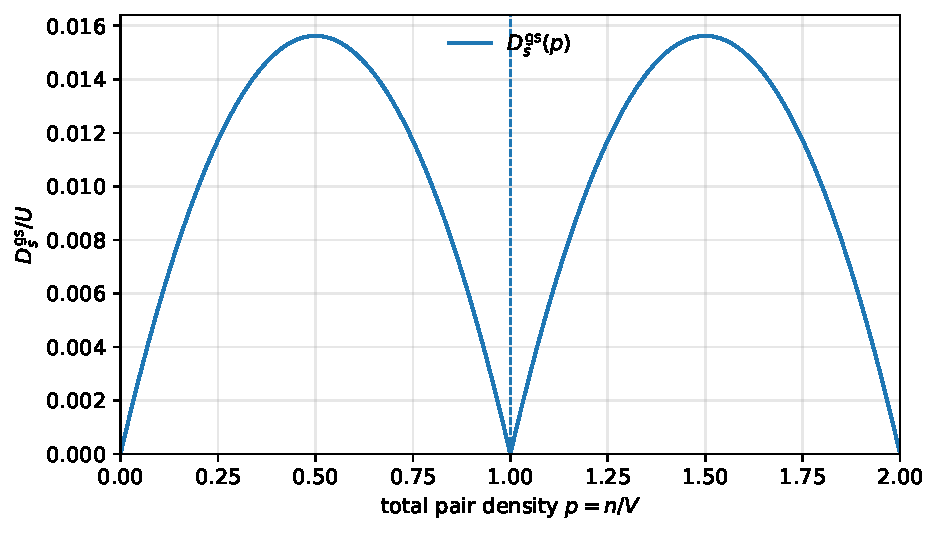
\includegraphics[width=0.76\linewidth]{figures/unresolved_response_gs.pdf}
\caption{Composition-relaxed ground-energy stiffness of the block-preserving model.  The middle zero is caused by block polarization into a full and an empty block, not by zero one-pair mobility.}
\label{fig:base-envelope}
\end{figure}

\begin{remark}[Static envelope versus dynamics]
Because $N_1$ and $N_2$ are exactly conserved in the base model, a state prepared in an interior composition does not dynamically relax to the endpoint minimizer.  Equation~\eqref{eq:base-thermo-envelope} is therefore an equilibrium ground-energy envelope, not by itself a theorem about the zero-frequency response of a system with finite relative-charge relaxation.
\end{remark}

\section{Why smooth common-unitary hybridization fails}
\label{sec:common-unitary}

A natural attempt to mix the two singular subbundles is a momentum-dependent sector rotation
\begin{equation}
\mathcal R_\gamma(\bmk)=
\begin{pmatrix}
\cos\gamma&\sin\gamma\,\e^{\I k_x}\\
-\sin\gamma\,\e^{-\I k_x}&\cos\gamma
\end{pmatrix}.
\label{eq:Rgamma}
\end{equation}
Conjugating the block-diagonal band Hamiltonian by $\mathcal R_\gamma\otimes\Id_2$ preserves the flat spectrum while creating momentum-dependent intersector hopping in the microscopic basis.  In the fixed zero-twist singular frame, a block-diagonal factor $s_\lambda=s_{\lambda,1}\oplus s_{\lambda,2}$ acquires the source
\begin{equation}
b_{\lambda i}=b_{\lambda i}^{\rm bp}
+G_i(\bmk)s_\lambda(\bmk,\bmk')
-s_\lambda(\bmk,\bmk')G_i(\bmk'),
\qquad
G_i=\mathcal R_\gamma^\dagger\partial_{k_i}\mathcal R_\gamma.
\label{eq:raw-common-source}
\end{equation}
Its $12$ block is generically nonzero.  Nevertheless, raw source mixing is not the physical curvature map.

\begin{proposition}[Common-unitary cancellation]
\label{prop:common-unitary}
Suppose an analytic twisted family has
\begin{equation}
S_{\lambda,\gamma}(\bmA)
=\widehat R(\bmA)S_{\lambda,{\rm bp}}(\bmA)
\widehat R(\bmA)^\dagger
\end{equation}
with the same unitary $\widehat R$ for every factor label.  Then the commutator contribution to the first source lies in $\operatorname{ran}D(0)$ on every zero mode.  It is annihilated by $\Pi$, and
\begin{equation}
T_i^{(\gamma)}=T_i^{({\rm bp})},
\qquad
Q_i^{(\gamma,n)}=Q_i^{({\rm bp},n)}.
\end{equation}
\end{proposition}

\begin{proof}
Let $\widehat G_i=\partial_{A_i}\widehat R|_0$.  On a zero mode $\ket\psi$,
\begin{equation}
[\widehat G_i,S_\lambda(0)]\ket\psi
=-S_\lambda(0)\widehat G_i\ket\psi.
\end{equation}
Collecting all factor labels gives $-D(0)\widehat G_i\ket\psi$, and $\Pi D(0)=0$.
\end{proof}

The obstruction is limited but decisive.  It rules out a shared smooth frame rotation as the origin of composition hopping.  It does not rule out a factor family whose full Peierls derivative is not a common covariance commutator.  A zero projected row is necessary for the simple source construction, but, as the next section shows, it is not sufficient when the factor kernel itself is multi-site and must twist covariantly.

\section{Twist covariance, displacement balance, and the conditional transfer operator}
\label{sec:twist-covariance}

\subsection{Covariant zero-row cancellation}

The Peierls prescription in \cref{sec:base-model} applies to every multi-site kernel, not only to the normal-state Hamiltonian.  For a neutral one-body operator
\begin{equation}
 B_{\bm R}(0)=\sum_{x,y}B_{\bm R}(x,y)c_x^\dagger c_y,
\end{equation}
its covering-lattice lift is
\begin{equation}
 B_{\bm R}(\bm A)=\sum_{x,y}B_{\bm R}(x,y)
 \e^{-\I\bm A\cdot(x-y)}c_x^\dagger c_y.
 \label{eq:bridge-peierls}
\end{equation}
Equivalently, in a translation-invariant Bloch representation its kernel is shifted as $B(\bmk;\bm A)=B(\bmk+\bm A)$.  The same shift acts on the isolated-band projector $P(\bm A)$.

\begin{proposition}[Covariant bridge cancellation]
\label{prop:covariant-bridge}
Let
\begin{equation*}
P(\bm A)=\widehat U(\bm A)P_0\widehat U(\bm A)^\dagger,
\qquad
B(\bm A)=\widehat U(\bm A)B_0\widehat U(\bm A)^\dagger
\end{equation*}
be generated by the same displacement-resolved Peierls lift.  Then
\begin{equation}
 P(\bm A)B(\bm A)P(\bm A)
 =\widehat U(\bm A)(P_0B_0P_0)\widehat U(\bm A)^\dagger.
 \label{eq:covariant-pbp}
\end{equation}
In particular, if $P_0B_0P_0=0$, the projected row vanishes for every $\bm A$ and has no first-order source.
\end{proposition}

\begin{proof}
Equation~\eqref{eq:covariant-pbp} follows by inserting the common conjugation.  Differentiating at zero gives
\begin{equation}
 (\partial_iP)B_0P_0+P_0(\partial_iB)P_0+P_0B_0(\partial_iP)
 =[G_i,P_0B_0P_0],
 \qquad G_i=\left.\partial_{A_i}\widehat U\right|_0,
\end{equation}
which is zero when the projected row is zero.  The middle term is precisely the contribution omitted when $B$ is held fixed while $P$ twists.
\end{proof}

This proposition is distinct from, but parallel to, the common-unitary cancellation of \cref{prop:common-unitary}.  A multi-site filtered bridge is not an external, twist-independent probe.  Its own displacement phases must be differentiated, and they cancel the projector-only source.

\subsection{Net displacement of a many-fermion vertex}

The correct microscopic invariant is the net displacement of the complete vertex.  Consider one normal-ordered charge-neutral monomial
\begin{equation}
 \mathcal O_{\bm x;\bm y}
 =C\,c_{\alpha_1,x_1}^\dagger\cdots c_{\alpha_m,x_m}^\dagger
 c_{\beta_m,y_m}\cdots c_{\beta_1,y_1}.
\end{equation}
Its uniform Peierls phase is
\begin{equation}
 \mathcal O_{\bm x;\bm y}(\bm A)
 =\e^{-\I\bm A\cdot\Delta\bm R}\mathcal O_{\bm x;\bm y}(0),
 \qquad
 \Delta\bm R=\sum_{j=1}^m x_j-\sum_{j=1}^m y_j.
 \label{eq:net-displacement-phase}
\end{equation}

\begin{theorem}[Displacement-balance criterion]
\label{thm:displacement-balance}
A nonzero monomial is invariant under every uniform vector potential if and only if its covering-lattice net displacement is zero.  A finite vertex is invariant termwise if and only if every monomial remaining after like terms are combined has $\Delta\bm R=0$.
\end{theorem}

The covering-lattice qualification is essential on a torus: winding-related aliases must be lifted before their displacement is tested.  A position-balanced pair hop is the canonical example,
\begin{equation}
 H_{\rm ph}=\sum_{x,x'}P_{xx'}
 c_{1x\uparrow}^\dagger c_{1x'\downarrow}^\dagger
 c_{2x'\downarrow}c_{2x\uparrow}+{\rm H.c.}
 \label{eq:position-balanced-pair-hop}
\end{equation}
For every term, the created and annihilated positions are the same unordered pair $\{x,x'\}$, so $\Delta\bm R=0$ exactly even though two fermions are transferred between blocks.

\subsection{Quadrature anisotropy is exactly pair transfer}

Let $X$ be a directed spin-preserving transfer and define
\begin{equation}
 B^X=X+X^\dagger,
 \qquad
 B^Y=-\I(X-X^\dagger).
\end{equation}
Then
\begin{equation}
 \boxed{
 \frac12\left[g_X^2(B^X)^2+g_Y^2(B^Y)^2\right]
 =\frac J2(XX^\dagger+X^\dagger X)
 -\frac{P_{\rm ph}}2(X^2+X^{\dagger2}),}
 \label{eq:quadrature-pair-transfer}
\end{equation}
where
\begin{equation}
 J=g_X^2+g_Y^2,
 \qquad
 P_{\rm ph}=g_Y^2-g_X^2.
 \label{eq:J-Pph-corrected}
\end{equation}
Thus $P_{\rm ph}$ multiplies precisely the pair-transfer component, up to the displayed sign convention.  Density/exchange terms live in $XX^\dagger+X^\dagger X$; coherent transfer of two fermions lives in $X^2+X^{\dagger2}$.  Equation~\eqref{eq:position-balanced-pair-hop} shows that a nonzero $P_{\rm ph}$ is fully compatible with Peierls covariance.  Position balance alone does not force $P_{\rm ph}=0$; it only guarantees that the complete vertex carries no explicit uniform-$\bm A$ phase.

\subsection{The compact paraunitary model as a covariance audit}

The finite-range normal-state construction remains useful, but its role changes.  Define
\begin{equation}
 \mathcal W(z)=\frac12
 \begin{pmatrix}1+z&1-z\\1-z&1+z\end{pmatrix},
 \qquad
 \mathcal D=\operatorname{diag}(1,\I),
\end{equation}
\begin{equation}
 \mathcal U_1(\bmk)=\mathcal W(\e^{\I k_x})\mathcal D\mathcal W(\e^{\I k_y}),
 \qquad
 \mathcal U_2(\bmk)=\mathcal W(\e^{\I k_y})\mathcal D\mathcal W(\e^{\I k_x}).
 \label{eq:compact-frames-revised}
\end{equation}
Writing $\mathcal U_a=(u_a,r_a)$, the active and bright Wannier functions have compact plaquette support.  Their averaged active-band metrics are
\begin{equation}
 \overline g_1=\begin{pmatrix}1/8&0\\0&1/4\end{pmatrix},
 \qquad
 \overline g_2=\begin{pmatrix}1/4&0\\0&1/8\end{pmatrix},
\end{equation}
and with the kernel $K$ of \cref{eq:base-QGN},
\begin{equation}
 m_{{\rm pair},1}^{-1}=U\begin{pmatrix}1/4&0\\0&1/2\end{pmatrix},
 \qquad
 m_{{\rm pair},2}^{-1}=U\begin{pmatrix}5/4&0\\0&5/8\end{pmatrix}.
 \label{eq:compact-masses-revised}
\end{equation}

Let $w_{a,\bm R,s}$ and $b_{a,\bm R,s}$ denote compact active and bright Wannier orbitals and put
\begin{equation}
 X_{\bm R}=\sum_s b_{1,\bm R,s}^\dagger w_{2,\bm R,s}.
\end{equation}
Because these Wannier orbitals have multi-cell support, $X_{\bm R}$ is a multi-site bilinear.  Holding its kernel fixed while twisting only $P(\bm A)$ gives the previously reported derivatives
\begin{equation}
 \left.\partial_{A_y}(PB_{\bm R}^XP)\right|_0=-\frac12B_{{\bm R},{\rm act}}^Y,
 \qquad
 \left.\partial_{A_y}(PB_{\bm R}^YP)\right|_0=\frac12B_{{\bm R},{\rm act}}^X.
 \label{eq:fixed-kernel-diagnostic}
\end{equation}
They are mathematically correct for a fixed external kernel, but not for the electromagnetic lift of this bridge.  With $X_{\bm R}(\bm A)$ Peierls shifted together with $P(\bm A)$,
\begin{equation}
 P(\bm A)B_{\bm R}^{X,Y}(\bm A)P(\bm A)=0
 \quad\text{for every }\bm A.
 \label{eq:compact-covariant-zero}
\end{equation}
The numerical audit in \cref{fig:bridge-covariance} displays the two conventions directly.

\begin{figure}[t]
\centering
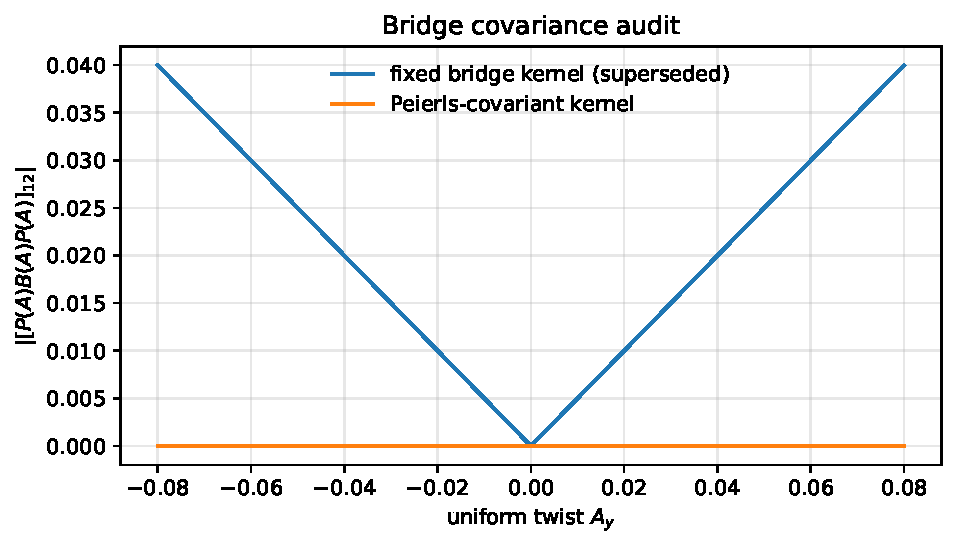
\includegraphics[width=0.78\linewidth]{figures/bridge_covariance_audit.pdf}
\caption{Projected compact bridge under a representative $A_y$ twist.  Holding the multi-site bridge kernel fixed produces the linear response used in the superseded verifier.  Shifting the bridge kernel as $B(\bmk+\bm A)$ together with the projector makes the projected row zero to machine precision for all $A_y$.}
\label{fig:bridge-covariance}
\end{figure}

\subsection{Conditional Jacobi reduction and two spectral consequences}

The Jacobi algebra derived from active transfer source vectors remains exact, but it must be stated conditionally.  Suppose a fully covariant microscopic model produces, after the target projection of \cref{eq:target-map}, the active transfer rows
\begin{equation}
 T_{y,X}=-\frac{g_X}{2}B_{\rm act}^Y,
 \qquad
 T_{y,Y}=\frac{g_Y}{2}B_{\rm act}^X.
 \label{eq:conditional-transfer-source}
\end{equation}
No claim is made here that the compact filtered bridge supplies these rows.  At fixed total pair number $n$, their source Gram plus the blockwise QGN curvature is the exact Jacobi matrix
\begin{equation}
 Q_y^{(n)}=
 \sum_{r=r_-}^{r_+}d_{r,y}\ket r\!\bra r
 +\sum_{r=r_-}^{r_+-1}t_{r,y}
 (\ket{r+1}\!\bra r+\ket r\!\bra{r+1}),
 \label{eq:conditional-Jacobi}
\end{equation}
where $r_-=\max(0,n-V)$, $r_+=\min(V,n)$ and
\begin{align}
 d_{r,y}={}&2U\rho_V(r)+\frac{5U}{2}\rho_V(n-r)\notag\\
 &+\frac{J}{2V}\left[(n-r)(V-r)+r(V-n+r)\right],
 \label{eq:conditional-Jacobi-diag}\\
 t_{r,y}={}&\frac{P_{\rm ph}}{2V}
 \sqrt{(n-r)(V-r)(r+1)(V-n+r+1)}.
 \label{eq:conditional-Jacobi-hop}
\end{align}
The off-diagonal is exactly the pair-transfer part of \cref{eq:quadrature-pair-transfer}.

\begin{lemma}[Transfer-dark zero mode]
\label{lem:transfer-dark}
For the bridge-source Gram alone ($U=0$) at $n=V$, if either $g_X=0$ or $g_Y=0$, then $Q_y^{(V)}$ has an exact zero mode.  Writing $\sigma=\operatorname{sgn}P_{\rm ph}$,
\begin{equation}
 \ket{\Omega_\sigma}=\mathcal N^{-1}
 \sum_{r=0}^V(-\sigma)^r\binom Vr\ket{r,V-r}
 \label{eq:transfer-dark-vector}
\end{equation}
obeys $Q_y^{(V)}\ket{\Omega_\sigma}=0$.
\end{lemma}

\begin{proof}
When one quadrature vanishes, $|P_{\rm ph}|=J$.  Dividing the three-term recurrence by $J/(2V)$, the diagonal coefficient is $(V-r)^2+r^2$ and the neighboring coefficients are $(V-r+1)r$ and $(V-r)(r+1)$.  The binomial ratios in \eqref{eq:transfer-dark-vector} cancel these three terms exactly.
\end{proof}

Thus the earlier warning that both quadratures should remain nonzero is an exact lemma, not merely a heuristic.  The positive blockwise curvature changes the large-volume result more substantially.

\begin{proposition}[Middle-filling thermodynamic stiffness]
\label{prop:middle-limit}
For the $y$-direction coefficients in \cref{eq:compact-masses-revised}, at $n=V$ and fixed $U,g_X,g_Y$,
\begin{equation}
 \boxed{
 \lim_{V\to\infty}\frac1{4V}\lambda_{\min}(Q_y^{(V)})
 =\frac18\min\left\{J,\ g_{\min}^2+\frac94U\right\},}
 \qquad g_{\min}^2=\min(g_X^2,g_Y^2).
 \label{eq:middle-limit}
\end{equation}
If
\begin{equation}
 U\ge\frac49\max(g_X^2,g_Y^2),
 \label{eq:endpoint-condition}
\end{equation}
then the minimizing states localize near the endpoint compositions and the limit improves to
\begin{equation}
 \lim_{V\to\infty}D_{s,y}^{\rm gs}(p=1)=\frac{J}{8}
 =\frac{g_X^2+g_Y^2}{8},
 \label{eq:J-over-eight}
\end{equation}
independent of $P_{\rm ph}$.
\end{proposition}

\begin{proof}
Set $x=r/V$.  The diagonal and off-diagonal coefficients of $Q_y^{(V)}/V$ converge to
\begin{equation}
 d(x)=\frac J2[x^2+(1-x)^2]+\frac92Ux(1-x),
 \qquad
 t(x)=\frac{P_{\rm ph}}2x(1-x).
\end{equation}
The lower symbol of the slowly varying Jacobi family is
\begin{equation}
 f(x)=d(x)-2|t(x)|
 =\frac J2+x(1-x)\left(\frac92U-J-|P_{\rm ph}|\right).
\end{equation}
Gershgorin lower bounds and localized trial vectors give
$\lambda_{\min}(Q_y^{(V)})/V\to\min_{x\in[0,1]}f(x)$.  If the parenthesis is nonnegative, the minimum is $J/2$ at $x=0,1$.  Otherwise it is attained at $x=1/2$ and equals $g_{\min}^2/2+9U/8$.  Division by four proves \eqref{eq:middle-limit}.  The endpoint condition is equivalent to $9U/2\ge J+|P_{\rm ph}|=2\max(g_X^2,g_Y^2)$.
\end{proof}

For the verifier parameters $U=1$, $g_X=0.8$, and $g_Y=0.3$, condition~\eqref{eq:endpoint-condition} holds and the finite-size sequence converges to $J/8=0.09125$, as shown in \cref{fig:middle-convergence}.

\begin{figure}[t]
\centering
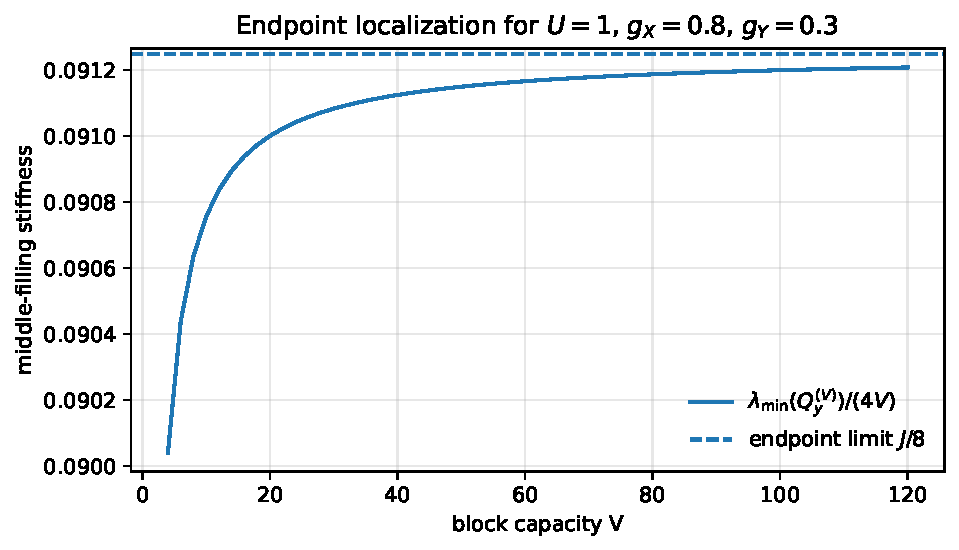
\includegraphics[width=0.76\linewidth]{figures/middle_stiffness_convergence.pdf}
\caption{Finite-capacity convergence of the conditional middle-filling Jacobi stiffness for the verifier parameters.  The endpoint-localized limit is $J/8$, independent of the sign and magnitude of $P_{\rm ph}$ within the endpoint regime.}
\label{fig:middle-convergence}
\end{figure}

\begin{table}[t]
\centering
\caption{Numerical covariance and conditional-Jacobi checks.}
\label{tab:covariance-verification}
\begin{tabular}{@{}lr@{}}
\toprule
Check & Maximum absolute error or residual\\
\midrule
Fixed-kernel derivative versus \eqref{eq:fixed-kernel-diagnostic} & $1.65\times10^{-10}$\\
Covariantly projected bridge value & $2.81\times10^{-16}$\\
Covariant finite-difference derivative & $1.99\times10^{-10}$\\
Direct Fock Gram versus conditional Jacobi formula & $1.1\times10^{-16}$\\
Transfer-dark zero-vector residual at $V=120$ & $3.8\times10^{-15}$\\
\bottomrule
\end{tabular}
\end{table}

The structural conclusion is deliberately narrower than the superseded bridge claim.  Position-balanced pair hopping supplies a gauge-consistent route to $P_{\rm ph}\ne0$, and \cref{eq:conditional-Jacobi} gives the exact many-body reduction once a legitimate transfer source is present.  Constructing a local microscopic factor whose covariant Peierls derivative survives the target projection remains an open realization problem.

\section{Material screen at \texorpdfstring{$3.65^\circ$ twisted bilayer WSe$_2$}{3.65-degree twisted bilayer WSe2}}
\label{sec:wse2-365}

\subsection{Three-orbital Wannier Hamiltonian and scales}

We reconstruct the published MX/MM/XM three-orbital Hamiltonian of Kim \emph{et al.}~\cite{kim2025}.  At zero displacement field its principal parameters are
\begin{equation}
\begin{aligned}
\delta&=-14.9~{\rm meV},&
 t_{TH}^{(1)}&=10.78~{\rm meV},&
 t_{HH}^{(1)}&=0.55~{\rm meV},\\
 t_{TT}^{(1)}&=-1.95~{\rm meV},&
 t_{TH}^{(2)}&=-1.21~{\rm meV},&
 t_{HH}^{(3)}&=5.4~{\rm meV},\\
 U_H&=35~{\rm meV},&
 U_T&=20~{\rm meV},&
 V&=40~{\rm meV},\qquad J=10~{\rm meV}.
\end{aligned}
\end{equation}
The reconstructed top, second, and remote bands have bandwidths
\begin{equation}
 W_1=29.9614~{\rm meV},\qquad
 W_2=19.1716~{\rm meV},\qquad
 W_r=22.1933~{\rm meV},
\end{equation}
and the minimum second-to-remote direct gap is $\Delta_{2r}=7.77326~{\rm meV}$.  An independent direct three-band Wannier construction has the minimal K-valley Chern sequence $(1,1,-2)$~\cite{tuo2025}.

\subsection{Active--remote geometry is a proxy, not a source}

For active band $a$ and remote band $r$, define the gauge-invariant interband metric contribution
\begin{equation}
 \gamma^{(r)}_{a,ij}
 =\left\langle\operatorname{Re}
 \frac{\langle u_a|\partial_{k_i}h|u_r\rangle
       \langle u_r|\partial_{k_j}h|u_a\rangle}
 {(E_a-E_r)^2}\right\rangle_{\bmk}.
\end{equation}
The reconstructed model gives
\begin{equation}
 \gamma_1^{(r)}=0.003129013\,a_M^2\Id_2,
 \qquad
 \gamma_2^{(r)}=0.222859185\,a_M^2\Id_2.
\end{equation}
The selected remote line supplies about $3.3\%$ of the top-band metric and $71.0\%$ of the second-band metric.  The legacy orbital/path weighting gives
\begin{equation}
 \Gamma_x^{\rm proxy}=\Gamma_y^{\rm proxy}=0.066805404\,a_M^2.
 \label{eq:material-Gamma-proxy}
\end{equation}
This number remains a useful measure of active--remote overlap and local-path compatibility.  By Proposition~\ref{prop:covariant-bridge}, however, it cannot be inserted as a physical source coefficient for a filtered multi-site bridge whose kernel is Peierls shifted together with the projector.

A bare local triangular--honeycomb bilinear is also not a zero row: its estimated active--active Hilbert--Schmidt leakage is about $0.463$ per bond, versus $0.0533$ in the desired remote-to-active component.  The real-space locality calculation therefore diagnoses how well a filtered object can be truncated, but it does not repair the covariance cancellation.

\subsection{Projected interactions and the position-balanced quadrature obstruction}

Projecting $U_H,U_T,V,J$ into singlet Cooper channels gives the spectral norms in \cref{tab:365-kernels}.
\begin{table}[H]
\centering
\caption{Spectral norms of the projected $3.65^\circ$ singlet Cooper kernels, in meV.}
\label{tab:365-kernels}
\begin{tabular}{@{}lrrrrrr@{}}
\toprule
Channel & $1\to1$ & $2\to2$ & $r\to r$ & $1\leftrightarrow2$ & $1\leftrightarrow r$ & $2\leftrightarrow r$\\
\midrule
$\|K\|$ & 27.0465 & 14.5707 & 25.4025 & 6.7337 & 9.9896 & 13.2353\\
\bottomrule
\end{tabular}
\end{table}
The normalized cross-channel ratios are $0.339$, $0.381$, and $0.688$, so the two highest energy bands are not exact interaction-preserved QGN blocks.

The Fierz decomposition of the published local tensor gives
\begin{equation}
 P_{\rm ph}=0,
 \qquad
 g_X^2=g_Y^2=J/2,
 \label{eq:UVJ-equal-quadratures-revised}
\end{equation}
and hence no pair-transfer component in \cref{eq:quadrature-pair-transfer}.  The microscopic $U,V,J$ monomials are position balanced: their created and annihilated positions have zero net displacement.  This explains why they require no independent Peierls phase, but position balance by itself is not the reason for equal quadratures.  Equality follows from the actual interaction tensor and its Fierz content.  A separate position-balanced pair hop of the form \eqref{eq:position-balanced-pair-hop} is symmetry allowed and would give $P_{\rm ph}\ne0$ without violating twist covariance.

The previously reported one-pair matrix and many-composition Fock agreement for a benchmark $P_{\rm ph}=2~{\rm meV}$ remain valid checks of the conditional Jacobi algebra in \cref{eq:conditional-Jacobi}.  They do \emph{not} establish a physical WSe$_2$ source, because the source rows were generated with the filtered bridge held fixed.  We therefore remove the earlier identification $t_{0,i}=2P_{\rm ph}\Gamma_i^{\rm proxy}$ from the material claim.

\subsection{Finite-bandwidth and remote-band corrections}

The ratios
\begin{equation}
 \frac{W_1}{\Delta_{2r}}=3.854,
 \qquad
 \frac{W_2}{\Delta_{2r}}=2.466,
 \qquad
 \frac{J}{\Delta_{2r}}=1.286
\end{equation}
are already too large for a controlled isolated-band limit.  The projected active--remote kernels give naive second-order scales
\begin{equation}
 \frac{\|K_{1r}\|^2}{\Delta_{2r}}\simeq12.84~{\rm meV},
 \qquad
 \frac{\|K_{2r}\|^2}{\Delta_{2r}}\simeq22.54~{\rm meV}.
\end{equation}
A displacement-field scan shows the same gap--geometry tradeoff found previously: fields that enlarge $\Delta_{2r}$ suppress the geometric proxy, and no scanned field makes both active bandwidths smaller than the remote gap.

The corrected $3.65^\circ$ conclusion is therefore
\begin{equation}
\boxed{
\begin{minipage}{0.86\linewidth}
Active--remote geometry is nonzero, but the filtered one-body bridge has no covariant source; the published $U,V,J$ tensor has $P_{\rm ph}=0$; the proposed energy-band blocks are strongly mixed; and the isolated-band expansion is uncontrolled.
\end{minipage}}
\end{equation}

\section{Interaction-defined singular subbundles}
\label{sec:interaction-subblocks}

The energy-band basis is not privileged by the interaction.  We therefore retain the interaction-Gram construction as a gauge-covariant block diagnostic, while separating its geometry from any claim about a physical source.

\subsection{Gauge-covariant interaction Gram operator}

Let $U_N(\bmk)$ contain an $N$-band composite energy manifold, and let $O_\lambda$ be local density and interlayer-transfer channels.  Their restrictions are
\begin{equation}
 F_\lambda(\bmk)=U_N^\dagger(\bmk)O_\lambda U_N(\bmk),
\end{equation}
and the positive interaction Gram operator is
\begin{equation}
 \boxed{\cS(\bmk)=\sum_\lambda g_\lambda
 F_\lambda^\dagger(\bmk)F_\lambda(\bmk).}
 \label{eq:material-interaction-Gram}
\end{equation}
If $\cS q_a=s_aq_a$, the physical singular projector is
\begin{equation}
 P_a(\bmk)=Q_a(\bmk)Q_a(\bmk)^\dagger,
 \qquad Q_a=U_Nq_a.
\end{equation}
A momentum-dependent basis change inside the composite manifold conjugates $\cS$ and leaves $P_a$ unchanged.

For a selected active pair $a,b$ and remote sector $r$, we monitor singular isolation $\delta_s$, two-band energy capture $C_{2E}$, the active--remote expectation gap $\Delta_{ar}$, normalized interaction leakage, and the screening ratio
\begin{equation}
 \epsilon_{\rm ctrl}^{(3)}=
 \frac{\max\{W_a,W_b,2\|H_{ab}\|_\infty,2\|H_{ar}\|_\infty,
 \sigma_{E,a},\sigma_{E,b}\}}{\Delta_{ar}}.
 \label{eq:threeband-control}
\end{equation}
This remains a ranking diagnostic, not a perturbative theorem.

\subsection{Projector finite differences and the precise \texorpdfstring{$\Gamma$}{Gamma} proxy}

The revised geometry code never differentiates a gauge-chosen singular vector.  On a mesh with step $\delta$ it uses
\begin{equation}
 D_iP_a(\bmk)=
 \frac{P_a(\bmk+\delta\hat e_i)-P_a(\bmk-\delta\hat e_i)}{2\delta},
 \label{eq:projector-difference}
\end{equation}
\begin{equation}
 g_{a,i}^{(\delta)}=\frac12\left\langle\Tr[(D_iP_a)^2]\right\rangle_{\bmk},
 \qquad
 \gamma_{ar,i}^{(\delta)}=
 \left\langle\Tr[P_r(D_iP_a)^2]\right\rangle_{\bmk}.
 \label{eq:projector-geometry}
\end{equation}
These expressions are phase independent and remain well defined in the low-$\delta_s$ regions where phase alignment becomes numerically fragile.

The three-band script contains local transfer operators $T_\ell$ for three paths.  For an ordered active mechanism $(a,b)$ define
\begin{equation}
 w_{\ell;br}(\bmk)=
 |\langle Q_r|T_\ell|Q_b\rangle|^2
 +|\langle Q_r|T_\ell^\dagger|Q_b\rangle|^2.
\end{equation}
The quantity reported by the archived max-over-path recipe is now defined explicitly as
\begin{equation}
 \boxed{
 \Gamma_i^{\max}=\frac1{a_M^2}
 \sum_{(a,b)=(1,2),(2,1)}
 \left\langle
 \Tr[P_r(D_iP_a)^2]\,
 \max_\ell w_{\ell;br}
 \right\rangle_{\bmk}.}
 \label{eq:Gamma-max-definition}
\end{equation}
It is a nonnegative, gauge-invariant geometric screening proxy.  It estimates simultaneous active--remote rotation and local-path overlap.  It is \emph{not} identified with $\|T_i\|^2$ or with a physical composition-hopping coefficient unless the derivative of the full covariant interaction factor is computed separately.

\subsection{Three-band exploratory and conservative scans}

The primary screen takes $N=3$ and uses top- and bottom-layer densities together with the $X$ and $Y$ quadratures of three local interlayer paths.  The exploratory domain contains $2800$ random points over
\begin{align}
2.0^\circ&\le\theta\le3.3^\circ,&
8&\le V\le16~{\rm meV},&
108^\circ&\le\psi\le150^\circ,\nonumber\\
8&\le w\le23~{\rm meV},&
0.40&\le m^*/m_e\le0.80,&
-12&\le V_z\le12~{\rm meV},
\end{align}
with transfer-channel weight $0\le\eta\le1$ and layer-density asymmetry $-0.4\le\delta_U\le0.4$.  A separate $1800$-point conservative scan stays near the standard lowest-order values.

After shell-$3$ refinement, 119 exploratory points remain valid and 94 satisfy the working control screen.  The strongest region favors lower twist angle, larger $V/w$, and heavier mass.  The upper score decile remains centered near $\theta\simeq2.18^\circ$, $V/w\simeq1.30$, and $m^*/m_e\simeq0.70$.

\begin{table}[t]
\centering
\caption{Projector-difference re-verification of the archived three-band representatives.  The last column is the geometric proxy \eqref{eq:Gamma-max-definition}; no $t_0$ is inferred.}
\label{tab:threeband-candidates}
\begin{tabular}{@{}lrrrrrr@{}}
\toprule
Candidate & $\theta$ & $\Delta_{ar}$ & $\delta_s$ & $C_{2E}$ & $\epsilon_{\rm ctrl}^{(3)}$ & $\Gamma_{\min}^{\max}$\\
& (deg) & (meV) &&&& ($a_M^2$ units)\\
\midrule
Balanced & 2.071 & 20.693 & 0.0902 & 0.9972 & 0.2526 & 0.003354\\
Maximum proxy & 2.286 & 12.397 & 0.1281 & 0.9705 & 0.9478 & 0.004013\\
Most controlled & 2.012 & 28.617 & 0.1874 & 0.9992 & 0.1322 & 0.001293\\
\bottomrule
\end{tabular}
\end{table}

The balanced representative has active widths about $1.75$ and $1.58$ meV, active--remote expectation gap $20.69$ meV, normalized active--active interaction leakage $0.0131$, and
\begin{equation}
 \Gamma_x^{\max}=0.00336078,
 \qquad
 \Gamma_y^{\max}=0.00335388
 \quad (a_M^2\text{ units}).
\end{equation}
The projector-difference values differ from the archived phase-aligned values by less than $2\times10^{-8}$ in this well-isolated representative, while removing the gauge sensitivity that matters closer to singular crossings.

\begin{figure}[t]
\centering
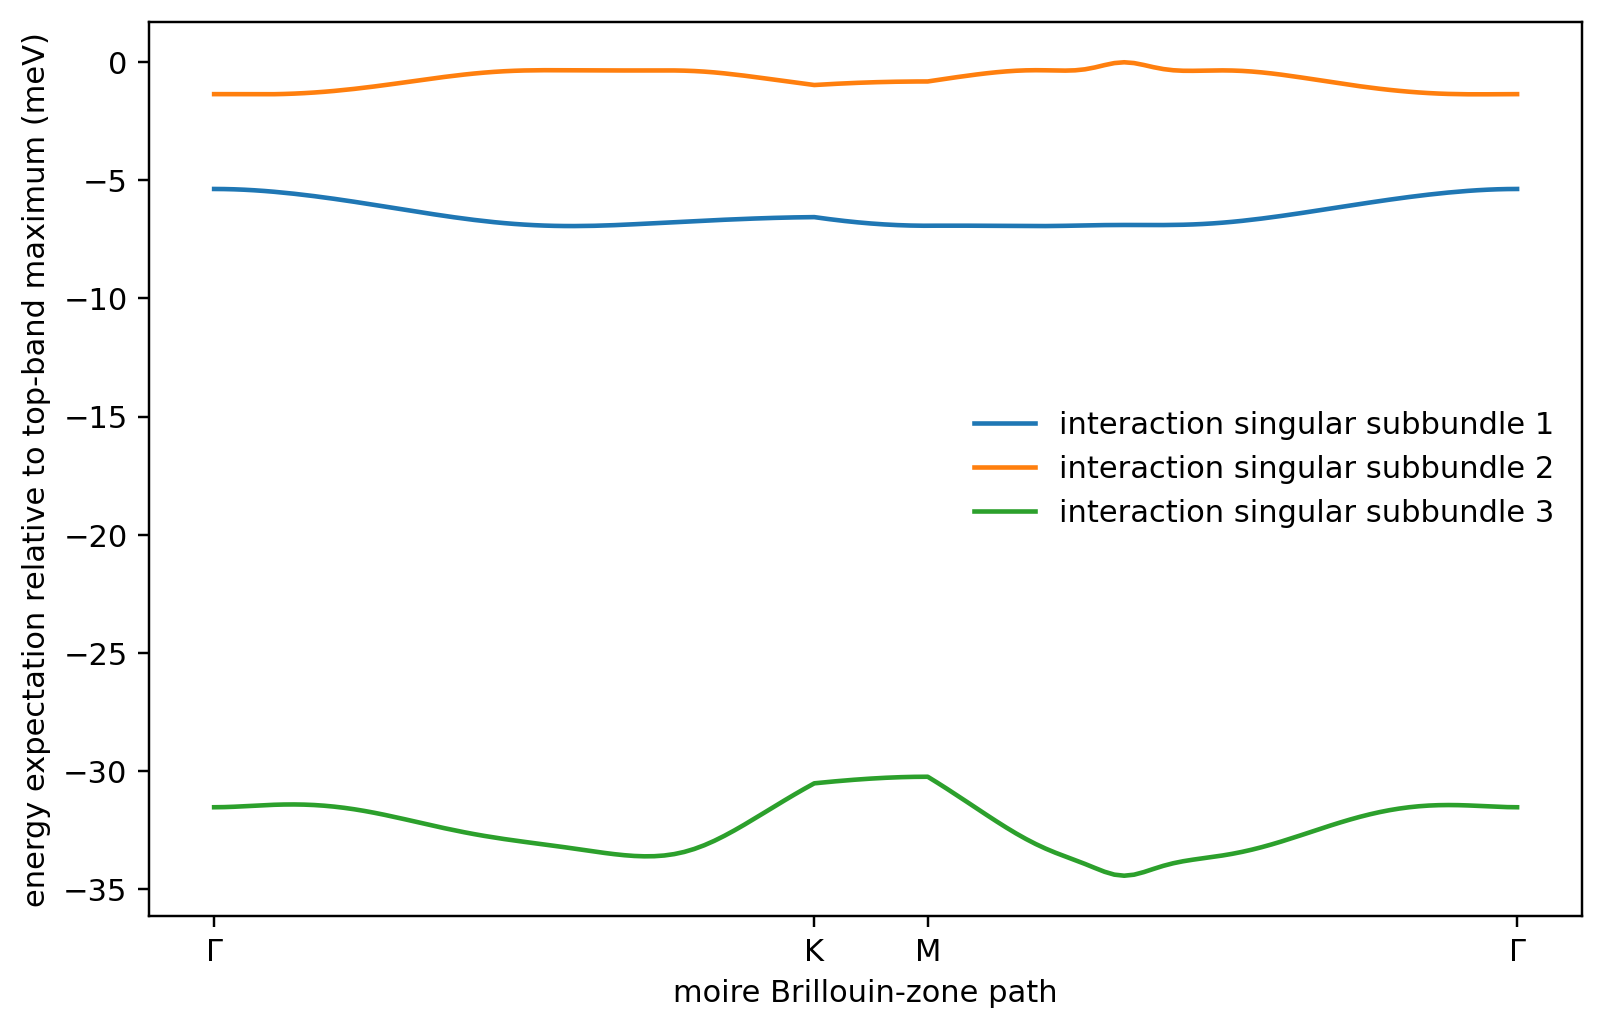
\includegraphics[width=0.86\linewidth]{figures/threeband_balanced_subbundles.png}
\caption{Energy expectations of the three interaction singular lines for the balanced three-band candidate.  The first two are selected as active and the third as the remote diagnostic sector.}
\label{fig:threeband-balanced}
\end{figure}

Holding the balanced point's remaining parameters fixed gives a narrow twist line: $\epsilon_{\rm ctrl}^{(3)}=0.224$ at $2.0^\circ$, $0.370$ at $2.1^\circ$, and $1.020$ at $2.2^\circ$.  Holding the standard lowest-order parameters fixed, no angle in $2^\circ$--$5^\circ$ satisfies all three-band controlled criteria.

\begin{figure}[t]
\centering
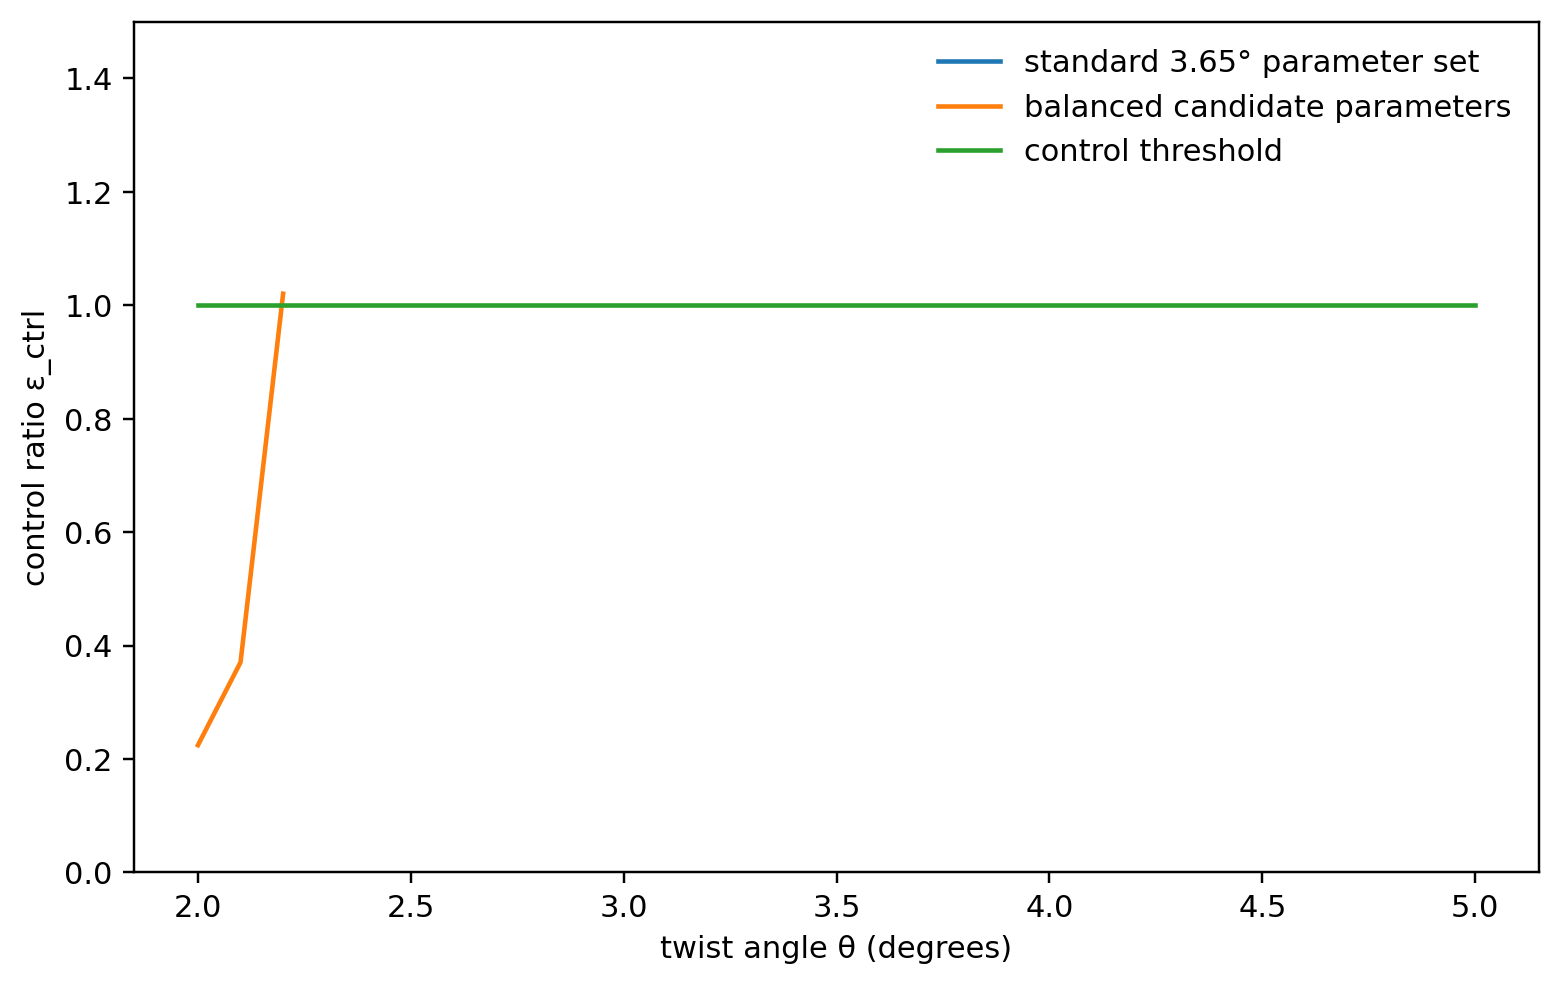
\includegraphics[width=0.80\linewidth]{figures/threeband_twist_control.png}
\caption{Twist-angle control ratio for the standard lowest-order parameter set and for the balanced candidate trajectory.  This remains a block-isolation and finite-bandwidth diagnostic, independent of the rejected fixed-bridge source.}
\label{fig:threeband-twist}
\end{figure}

\subsection{Four-band robustness scan}

A second scan enlarges the composite manifold to the top four energy bands, selects two leading interaction singular lines, and treats the remaining two directions as a remote complement.  Its geometry already uses projector differences.  The control error is normalized by the ambient gap from the four-band window to the fifth band and includes mixing into the two-dimensional remote sector.

The literature-anchored domain contains $3261$ coarse calculations over $2^\circ$--$5^\circ$.  No point passes the working interaction and control screen.  The best retained point has
\begin{equation}
 \theta=2.025^\circ,
 \qquad
 \epsilon_{\rm QGN}^{(4)}=0.229,
 \qquad
 \epsilon_{\rm ctrl}^{(4)}=5.930.
\end{equation}
An exploratory $1.2^\circ$--$3.2^\circ$ scan finds a near-threshold design point at
\begin{equation}
 \theta=1.2835^\circ,
 \qquad
 \epsilon_{\rm QGN}^{(4)}=0.0833,
 \qquad
 \epsilon_{\rm ctrl}^{(4)}=1.1368,
\end{equation}
with geometric proxies $\Gamma_x=0.03165$ and $\Gamma_y=0.02324$ in $a_M^2$ units.  It lies below the range in which the transferable model has been benchmarked against DFT and remains above the chosen control threshold.

The disagreement between the three- and four-band screens remains a principal numerical result.  Interaction-defined blocks can reduce leakage and identify a low-angle design direction, but neither screen now claims ordinary-twist composition hopping.  A material claim requires a fixed composite manifold, a covariantly projected interaction tensor, and the actual target-projected source map $T_i$.

\section{Discussion}
\label{sec:discussion}

\subsection{What is solved after the covariance correction}

The block-preserving part of the physical two-block program is complete.  The projected Hamiltonian, displacement-resolved Peierls lift, product-pseudospin zero space, exact pair branches, block masses, trace cancellation, and composition-relaxed middle zero are all explicitly derived.

The composition-mixing part now has two exact no-go statements.  A shared momentum-dependent unitary contributes only a removable commutator source.  A multi-site zero-row bridge that is Peierls shifted with the projector is a covariance orbit and remains zero.  These results sharply constrain future constructions: a legitimate source cannot be manufactured by twisting only a selected part of a covariant operator.

Two positive structural results survive.  First, the net-displacement theorem classifies which four-fermion vertices are exactly invariant under the uniform twist.  Second, the quadrature decomposition identifies $P_{\rm ph}$ with pair transfer and the conditional Jacobi reduction determines the complete many-composition response once a genuine source is supplied.  The transfer-dark lemma and the thermodynamic formula \eqref{eq:middle-limit} strengthen that algebraic result.

\subsection{What position balance does and does not prove}

Position balance proves that a vertex carries no explicit Peierls phase.  It does not imply equal quadratures, nor does it create a first-order source.  A position-balanced pair hop can give $P_{\rm ph}\ne0$, but the source map still depends on how the full interaction and band projectors vary under the physical twist.  The two ingredients must therefore be kept separate:
\begin{equation}
 \boxed{
 \text{composition hopping requires both a genuine }T_i\ne0
 \text{ and a pair-transfer component }P_{\rm ph}\ne0.}
 \label{eq:revised-core-criterion}
\end{equation}
A geometric overlap proxy such as $\Gamma_i^{\max}$ can help locate where $T_i$ might be large, but it cannot replace its direct calculation.

\subsection{Material interpretation}

Twisted WSe$_2$ remains a credible search platform because it supplies multiple local orbitals, nearby remote bands, and experimentally observed superconductivity over a range of twist angles~\cite{xia2025,guo2026}.  The interaction-SVD scans still show that singular subbundles are more natural QGN blocks than individual energy bands.  The low-angle direction also remains consistent with the appearance of a second flat Chern band in a relaxation-aware continuum model~\cite{zhang2025}.

The corrected claims are nevertheless more conservative.  The broad scans vary continuum parameters independently rather than along a relaxed material trajectory.  The three- and four-band diagnostics disagree on control.  Most importantly, the public $U,V,J$ tensor yields $P_{\rm ph}=0$, while no covariant source map has yet been extracted from a single microscopic interaction tensor.  Reported $\Gamma$ values are therefore design diagnostics, not stiffness predictions.

\subsection{Remaining open problems}

The next calculations should:
\begin{enumerate}
\item derive $\partial_{A_i}D(\bm A)$ from a single displacement-resolved microscopic interaction tensor, twisting every one- and many-body kernel consistently;
\item search for local factor families whose first derivative is not a common covariance commutator and survives the target projection;
\item extract position-balanced pair-transfer amplitudes together with density and exchange channels, rather than imposing $P_{\rm ph}$;
\item apply the interaction-Gram construction to a relaxation-aware WSe$_2$ continuum model in a converged multi-band manifold;
\item compute sewing-corrected topology and Wilson loops from projector data;
\item compare the conditional Jacobi reduction with direct finite-bandwidth many-body calculations after a legitimate source is found;
\item determine the dynamical zero-frequency response and the relevant order of limits.
\end{enumerate}

\section{Conclusion}

We have revised the physical two-block QGN program at its most delicate point: the electromagnetic covariance of a multi-site bridge.  The block-preserving model and its exact stiffness laws remain intact.  The proposed compact bridge source does not.  When the bridge kernel is Peierls shifted consistently with the projector, its zero row remains zero and the source cancels exactly.

The correction yields a clearer theory.  Uniform-twist invariance is controlled by net displacement of the complete many-fermion vertex.  Pair-transfer anisotropy is precisely the coefficient of $X^2+X^{\dagger2}$, and position-balanced pair hops can carry it without violating gauge covariance.  The finite Jacobi reduction is therefore retained as an exact conditional theorem, augmented by an exact transfer-dark zero mode and the middle-filling limit \eqref{eq:middle-limit}.

The WSe$_2$ screens now have an appropriately limited role.  They identify interaction-defined blocks, active--remote geometry, and low-angle control trends.  They do not establish a physical ordinary-twist source.  The material problem has been reduced to a sharper target: compute the fully covariant source map and the position-balanced pair-transfer tensor in the same microscopic model.

\begin{quote}
A nonzero geometric proxy and a nonzero pair-hop anisotropy are necessary design ingredients, but physical composition-space stiffness is claimed only after the complete Peierls-covariant source survives the target projection.
\end{quote}

\appendix

\section{Finite-torus displacement moments}
\label{app:lift}

For a displacement-resolved coefficient $X_\infty(\bm d)$, the physical torus lift is
\begin{equation}
X_{\bm N}(\bar{\bm d};\bm A)=
\sum_{\bm m\in\mathbb Z^2}
X_\infty(\bar{\bm d}+\bm m\odot\bm N)
\e^{-\I\bm A\cdot(\bar{\bm d}+\bm m\odot\bm N)}.
\end{equation}
At zero twist only the alias sum is visible.  Its first two derivatives are the unreduced displacement moments
\begin{align}
\left.\partial_{A_i}X_{\bm N}\right|_0
&=-\I\sum_{\bm m}d_{\bm m,i}X_\infty(\bm d_{\bm m}),\\
\left.\partial_{A_i}\partial_{A_j}X_{\bm N}\right|_0
&=-\sum_{\bm m}d_{\bm m,i}d_{\bm m,j}X_\infty(\bm d_{\bm m}).
\end{align}
The same lift must be applied to bridge kernels and many-fermion vertices before their twist derivatives are compared.

\section{Universal transfer factors}
\label{app:transfer}

The one-body reduced density matrix of a normalized capacity-$V$ block AGP is
\begin{equation}
\langle n_a|c_{a,i}^\dagger c_{a,j}|n_a\rangle
=\frac{n_a}{V}\delta_{ij}.
\end{equation}
For a transfer matrix $x:\cH_2\to\cH_1$ and $B_x=c_1^\dagger xc_2$, product structure gives
\begin{equation}
\langle B_y\bm n|B_x\bm n\rangle
=\frac{n_2}{V}\left(1-\frac{n_1}{V}\right)\Tr(y^\dagger x).
\end{equation}
Relative to one-pair normalization $V^{-1}\Tr(y^\dagger x)$ this yields
\begin{equation}
\tau_{1\leftarrow2}=\frac{n_2(V-n_1)}{V}.
\end{equation}
The overlap between opposite transfer directions from neighboring compositions is
\begin{equation}
\frac1V\sqrt{n_2(V-n_1)(n_1+1)(V-n_2+1)},
\end{equation}
which gives \cref{eq:clebsch-transfer}.

\section{Quadrature algebra and the transfer-dark vector}
\label{app:quadrature}

Expanding the Hermitian quadratures gives
\begin{align}
(B^X)^2&=X^2+X^{\dagger2}+XX^\dagger+X^\dagger X,\\
(B^Y)^2&=-X^2-X^{\dagger2}+XX^\dagger+X^\dagger X,
\end{align}
which proves \cref{eq:quadrature-pair-transfer}.  At $n=V$ and $U=0$, the Jacobi recurrence for a zero vector $v_r$ is
\begin{equation}
[(V-r)^2+r^2]v_r
+\sigma(V-r+1)r\,v_{r-1}
+\sigma(V-r)(r+1)v_{r+1}=0,
\end{equation}
where $\sigma=P_{\rm ph}/J=\pm1$.  The binomial vector
$v_r=(-\sigma)^r\binom Vr$ solves it term by term.

For the thermodynamic limit, the Gershgorin estimate
\begin{equation}
\lambda_{\min}(Q_V)\ge
\min_r\{d_r-|t_{r-1}|-|t_r|\}
\end{equation}
converges to $\min_x[d(x)-2|t(x)|]$.  Trial vectors supported in windows of width $o(V)$ around the minimizing $x$ and with the phase that makes the off-diagonal negative give the matching upper bound.  This supplies the standard Jacobi-family justification used in Proposition~\ref{prop:middle-limit}.

\section{Gauge-invariant projector geometry}
\label{app:projector-geometry}

For an isolated rank-one singular line, $P_a=|Q_a\rangle\langle Q_a|$ and
\begin{equation}
\frac12\Tr[(\partial_iP_a)^2]
=\langle\partial_iQ_a|(1-P_a)|\partial_iQ_a\rangle.
\end{equation}
For a distinct rank-one remote line,
\begin{equation}
\Tr[P_r(\partial_iP_a)^2]
=|\langle Q_r|\partial_iQ_a\rangle|^2.
\end{equation}
Thus \cref{eq:projector-difference,eq:projector-geometry} converge to the familiar vector formulas without choosing phases.  The code records the step $\delta$, the minimum singular gap, and the projector-difference method in every geometry result.

\section{Reproducibility map}
\label{app:reproducibility}

The revised archive contains:
\begin{enumerate}
\item \path{check_bridge_covariance.py}, which compares the fixed-kernel and covariant-kernel bridge derivatives, checks displacement balance, verifies the transfer-dark zero vector, and tests the finite-size middle-filling limit through $V=120$;
\item \path{interaction_singular_subbundle_scan_revised.py}, which replaces phase-aligned vector derivatives by projector differences and writes the exact max-over-path definition of $\Gamma_i^{\max}$ into its output;
\item \path{check_projector_geometry_convergence.py}, which repeats all three archived candidates at three steps,
$\delta/|\bm b_1|\in\{10^{-3},2\times10^{-3},4\times10^{-3}\}$.  The largest change from the middle step is below $5\times10^{-7}$ in the reported $\Gamma$ proxy;
\item machine-readable covariance, projector-reverification, and step-convergence files;
\item the legacy fixed-bridge verifier, retained only to document which algebraic calculation was superseded.
\end{enumerate}
The revised three-band representatives reproduce the archived geometric values in their well-isolated regime, but all $2P_{\rm ph}\Gamma_i$ quantities are labeled conditional proxies.  No script treats them as physical hopping coefficients after the covariance audit.

\begin{thebibliography}{99}

\bibitem{han2024}
Z. Han, J. Herzog-Arbeitman, B. A. Bernevig, and S. A. Kivelson,
``Quantum Geometric Nesting and Solvable Model Flat-Band Systems,''
\emph{Phys. Rev. X} \textbf{14}, 041004 (2024).

\bibitem{gao2026}
Q. Gao, Z. Han, and E. Khalaf,
``Bootstrapping Flatband Superconductors: Rigorous Lower Bounds on Superfluid Stiffness,''
\emph{Phys. Rev. Lett.} \textbf{136}, 076503 (2026).

\bibitem{parent}
N. Sledgianowski,
``Exact Flat-Band Stiffness from Pair Mobility in a QGN Model: Finite-size obstructions, a many-body reduction theorem, and a proof of the Gao--Han--Khalaf formula for Model II,'' manuscript (2026).

\bibitem{addendum}
N. Sledgianowski,
``Multi-Block Reduction and Irreducibility Laws for QGN Superconductors,'' manuscript (2026).

\bibitem{xia2025}
Y. Xia, Z. Han, K. Watanabe, T. Taniguchi, J. Shan, and K. F. Mak,
``Superconductivity in twisted bilayer WSe$_2$,''
\emph{Nature} \textbf{637}, 833--838 (2025).

\bibitem{guo2026}
Y. Guo, J. Cenker, A. Fischer, \emph{et al.},
``Angle evolution of the superconducting phase diagram in twisted bilayer WSe$_2$,''
\emph{Nature} \textbf{652}, 622--627 (2026).

\bibitem{kim2025}
S. Kim, J. F. Mendez-Valderrama, X. Wang, \emph{et al.},
``Theory of correlated insulators and superconductor at $\nu=1$ in twisted WSe$_2$,''
\emph{Nature Communications} \textbf{16}, 1701 (2025).

\bibitem{tuo2025}
C. Tuo, M.-R. Li, Z. Wu, W. Sun, and H. Yao,
``Theory of topological superconductivity and antiferromagnetic correlated insulators in twisted bilayer WSe$_2$,''
\emph{Nature Communications} \textbf{16}, 9525 (2025).

\bibitem{zhang2025}
X.-W. Zhang, K. Yang, C. Wang, X. Liu, T. Cao, and D. Xiao,
``Twist-angle transferable continuum model and second flat Chern band in twisted MoTe$_2$ and WSe$_2$,''
\emph{npj Quantum Materials} \textbf{10}, 110 (2025).

\bibitem{devakul2021}
T. Devakul, V. Cr\'epel, Y. Zhang, and L. Fu,
``Magic in twisted transition metal dichalcogenide bilayers,''
\emph{Nature Communications} \textbf{12}, 6730 (2021).

\bibitem{crepel2024}
V. Cr\'epel and A. Millis,
``Bridging the small and large in twisted transition metal dichalcogenide homobilayers: A tight binding model capturing orbital interference and topology across a wide range of twist angles,''
\emph{Phys. Rev. Research} \textbf{6}, 033127 (2024).

\bibitem{tovmasyan2016}
M. Tovmasyan, S. Peotta, P. T\"orm\"a, and S. D. Huber,
``Effective theory and emergent SU(2) symmetry in the flat bands of attractive Hubbard models,''
\emph{Phys. Rev. B} \textbf{94}, 245149 (2016).

\bibitem{huhtinen2022}
K.-E. Huhtinen, J. Herzog-Arbeitman, A. Chew, B. A. Bernevig, and P. T\"orm\"a,
``Revisiting flat band superconductivity: Dependence on minimal quantum metric and band touchings,''
\emph{Phys. Rev. B} \textbf{106}, 014518 (2022).

\bibitem{kohn1964}
W. Kohn,
``Theory of the insulating state,''
\emph{Phys. Rev.} \textbf{133}, A171--A181 (1964).

\bibitem{kato}
T. Kato, \emph{Perturbation Theory for Linear Operators}, 2nd ed. (Springer, Berlin, 1976).

\end{thebibliography}

\end{document}
